\begin{figure}[!ht]
	\centering
		\begin{subfigure}[t]{.3\textwidth}
			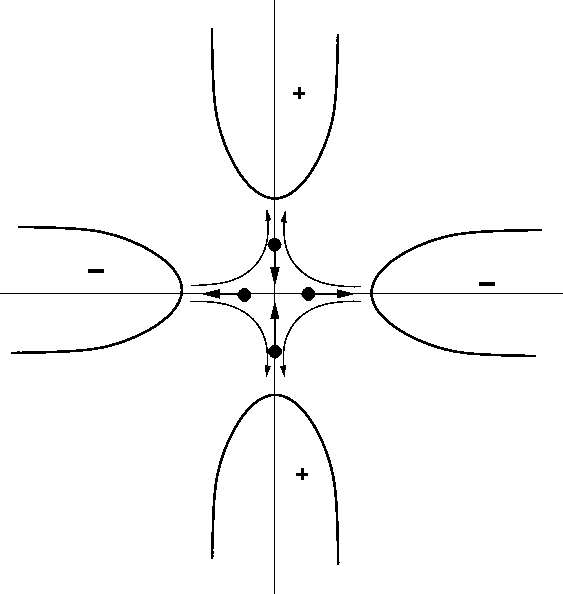
\includegraphics[width=\textwidth]{02_BeamDiag/figures/fig000_RFQ_a}
			\caption{Cut view of the transverse field.}
			\label{}
		\end{subfigure}
  ~
	\begin{subfigure}[t]{0.3\textwidth}
    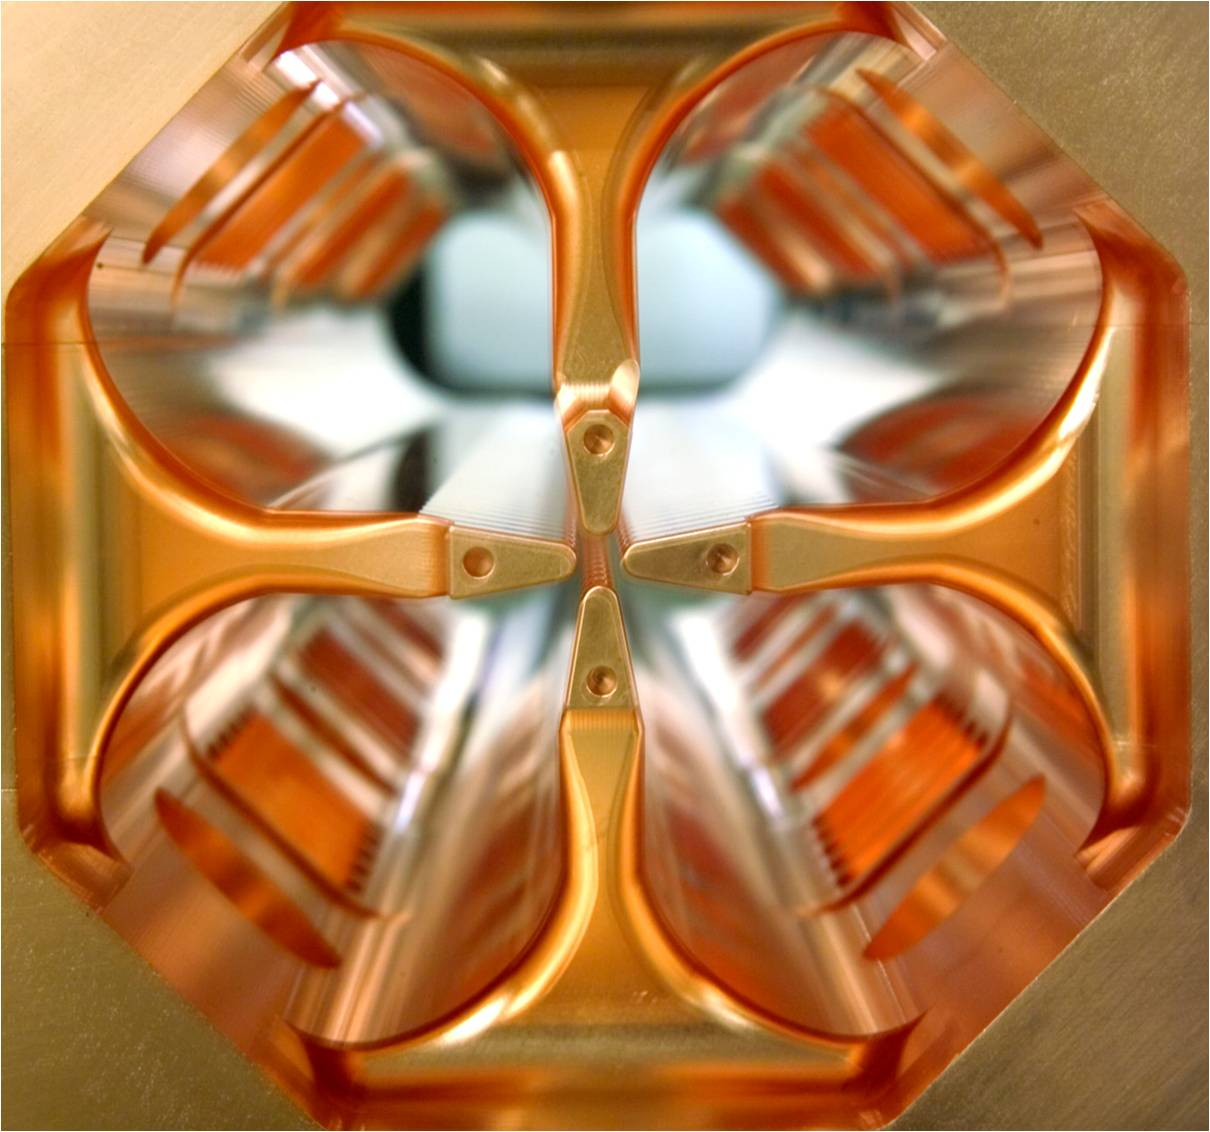
\includegraphics[width=\textwidth]{02_BeamDiag/figures/fig000_RFQ_b}
		\caption{Longitudinal modulation leading to an accelerating field.}
		\label{}
	\end{subfigure}
	~
	\begin{subfigure}[t]{0.3\textwidth}
		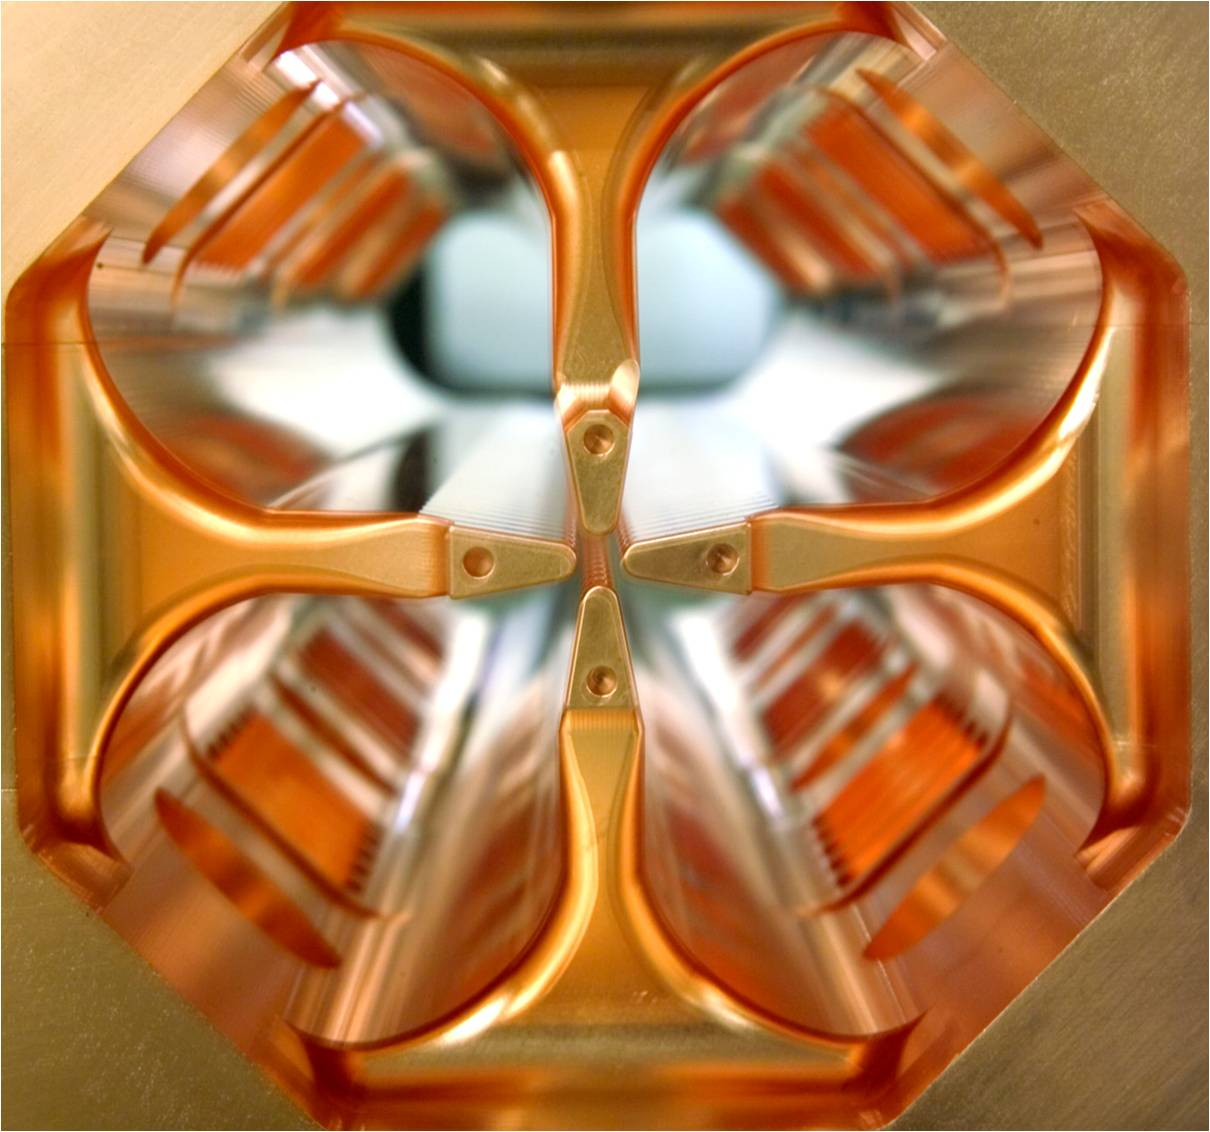
\includegraphics[width=\textwidth]{02_BeamDiag/figures/fig000_RFQ_c}
		\caption{The four vanes.}
		\label{}
	\end{subfigure}
	\caption[]{}
	\label{chap2:fig:RFQ}
\end{figure}
